Dans une salle d'escalade, un nouveau module en forme de tétraèdre, destiné à être posé au sol, est en cours de fabrication.

	Ce module servira à créer des plans inclinés.

	\smallskip

	On munit l'espace d'un repère orthonormé $\left(\mathrm{A} ; \vect{\imath}, \vect{\jmath}, \vect{k}\right)$.

	L'unité est le mètre.

	\smallskip

	On considère les trois points suivants : \quad B$\left(\dfrac{9}{2} ; 0 ; 0\right)$,\quad C$\left(\dfrac{9}{4} ; 3 ; 0\right)$ \quad et  \quad $D\left(\dfrac{3}{2} ; 1 ; 3\right)$.

	On modélise le module par le tétraèdre ABCD.

	On souhaite analyser ce module pour des raisons de construction et de sécurité.

	\begin{center}
	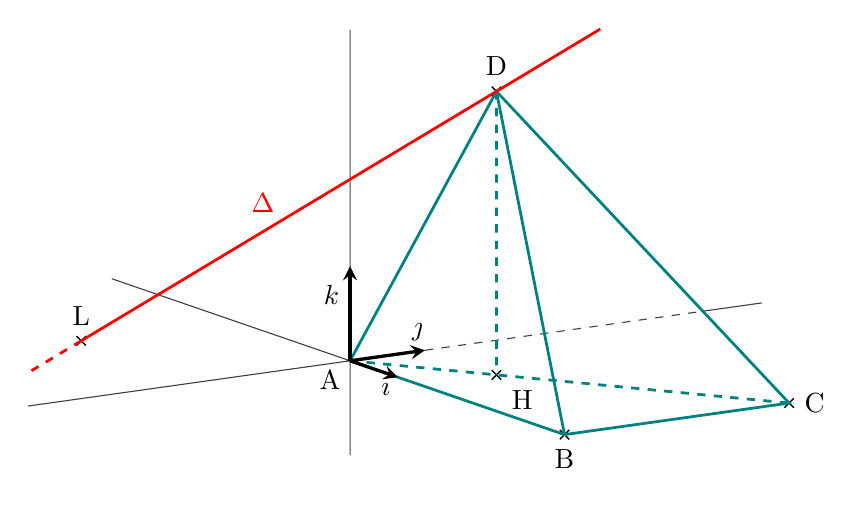
\begin{tikzpicture}[x=(-19:8mm),y=(8:12mm),z=(90:15mm),>=stealth,baseline={(current bounding box.center)},scale=0.8]
		\draw[darkgray] (-5,0,0) --(4.5,0,0)
			(0,-4.3,0)--(0,0,0) (0,4.69,0)--(0,5.5,0)
			(0,0,-1)--(0,0,3.5);
		\draw[darkgray,dashed] (0,1,0) -- (0,4.7,0);
		\foreach \coord/\nom/\pos in {{(4.5,0,0)}/B/{below}, {(4.5,3,0)}/C/{right}, {(1.5,1,3)}/D/{above}, {(1.5,1,0)}/H/{below right}, {(-2.5,-2,0)}/L/{above}}
		{\draw[shift={\coord},line width=0.5pt] (-45:3pt)--(135:3pt) (45:3pt)--(-135:3pt) (0,0,0) circle (0.1pt) node[\pos=2pt] {\nom} ;}
		\draw[teal,line width=1pt](0,0,0)--(4.5,0,0)--(4.5,3,0)--(1.5,1,3)--cycle
		 	(4.5,0,0)--(1.5,1,3);
	 	\draw[teal,line width=1pt,dashed](0,0,0)--(4.5,3,0) (1.5,1,3)--(1.5,1,0);
	 	\draw[red,line width=1pt] (-2.5,-2,0) -- (2.5,1.75,3.75) node[pos=0.35,above=3pt]{$\Delta$} ;
	 	\draw[red,line width=1pt,dashed](-2.5,-2,0)--(-3.,-2.375,-0.375) ;
	 	\draw[->,line width=1.2pt] (0,0,0)--(1,0,0) node[pos=0.75,below]{$\vect{\imath}$} ;
	 	\draw[->,line width=1.2pt] (0,0,0)--(0,1,0) node[pos=0.9,above]{$\vect{\jmath}$} ;
	 	\draw[->,line width=1.2pt] (0,0,0)--(0,0,1) node[pos=0.7,left]{$\vect{k}$} ;
	 	\node at(0,0,0) [below left] {A};
	\end{tikzpicture}
	\end{center}

	\subsection*{Partie A}
		\begin{enumerate}
			\item \begin{minipage}[t]{0.5\linewidth}
				On représente ci-contre le triangle ABC et sa hauteur issue de C.

				\begin{enumerate}
					\item Montrer que le triangle  ABC est isocèle en C.

					\item Montrer que l'aire du triangle  ABC est égale à $\np[m^2]{6,75}$.
				\end{enumerate}
			\end{minipage}
			\hfill
			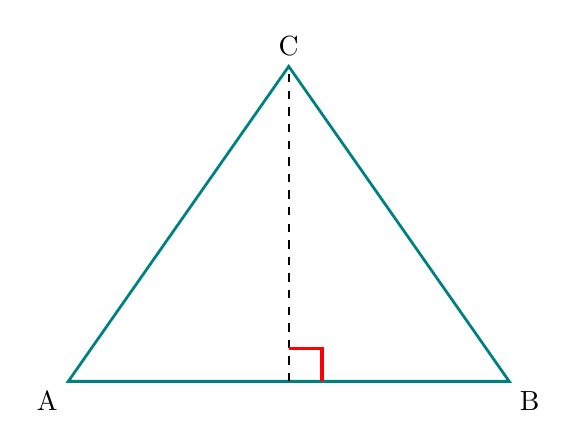
\begin{tikzpicture}[every node/.style={black},baseline={(C.base)}]
				\draw[line width=1pt,teal] (-2.8,0)node[below left]{A}--
				(2.8,0)node[below right]{B}--
				(0,4)node[above](C){C} -- cycle ;
				\draw[thick,dashed] (0,0)--(0,4);
				\draw[very thick,red] (0,12pt)--(12pt,12pt)--(12pt,0);
			\end{tikzpicture}

			\item \begin{enumerate}
				\item Vérifier qu'une équation cartésienne du plan (ABC) est :\quad $z=0$.

				\item Montrer que le point H$\left(\dfrac{3}{2} ; 1 ; 0\right)$ est le projeté orthogonal du point D sur le plan (ABC).
			\end{enumerate}

			\item On rappelle que le volume $\mathcal{V}$ d'un tétraèdre est donné par \quad $\mathcal{V} = \dfrac{1}{3} \times \mathcal{B} \times h$,\quad où $\mathcal{B}$ est l'aire d'une base et $h$ la hauteur relative à la base $\mathcal{B}$.

			En déduire le volume du module.
		\end{enumerate}



			\subsection*{Partie B}
		\begin{enumerate}
			\item On considère le vecteur $\vect{n}\begin{pmatrix} 4\\3\\3 \end{pmatrix}$.
			\begin{enumerate}
				\item Montrer que le vecteur $\vect{n}$ est un vecteur normal au plan (BCD).

				\item En déduire qu'une équation cartésienne du plan (BCD) est :
				\[4x+3y+3z-18=0.\]

				\item Donner une représentation paramétrique de la droite $\Delta$ orthogonale au plan (BCD) et passant par D.
			\end{enumerate}


			\item On admet que la droite $\Delta$ et le plan (ABC) sont sécants et on désigne par L leur point d'intersection.

			Montrer que L a pour coordonnées $\left(-\dfrac{5}{2} ; -2 ; 0\right)$.

			\item Le module est considéré adapté aux débutants si l'angle $\widehat{\mathrm{LDH}}$ est strictement inférieur à $60$\,\textdegree{}.

			Montrer que ce module est adapté aux débutants.
		\end{enumerate}
